\chapter{Eksperiment dokumentation}
I dette bilag beskrives fremgangsmåden for det foretagne forsøg samt findes data for forsøg.
\section{Fremgangsmåde}\label{appsec:sample-prep}
\subsection{Prøvefremstilling}
Til forsøget blev brugt fire prøver, hvoraf to var falske. De falske honning blev produceret selv, og indholdet kan ses i \cref{tab:samples}.
De fire prøver blev blandet ud fra masseforholdende i tabellen og ca. \qty{5}{\gram}\footnotemark{} blev overført til hver deres \qty{10}{\milli\liter} målekolbe.
\footnotetext{De eksakte afmålte værdier fremgår i \cref{tab:samples}.}
Der blev tilført \qty{4}{\milli\liter} \qty{20}{\milli\molar} \ch{HCl} til hvert af de fire glas med en mikropipette.
Derefter blev honning opløst ved hjælp af en vortex mixer, ved ca. \qty{2500}{\rpm}.
Måleglassene blev fyldt op til \qty{10}{\milli\liter} mærket med \qty{20}{\milli\molar} \ch{HCl} med en pasteurpipette i glas.
\subsection{Fastfaseekstraktion}
En vakuummanifold blev sat op med fire opsamlingsglas og fire kationbytterkolonner (Strata SCX, \qty{100}{\milli\gram}) sættes på over glassene.
Der blev med mikropipette tilsat, til hver kolonne, først \qty{1.0}{\milli\liter} methanol, derefter \qty{1.0}{\milli\liter} \qty{0.1}{\molar} \ch{HCl} og til slut \qty{1.0}{\milli\liter} demineraliseret vand uden at køre kolonnen tør.
\qty{0.50}{\milli\liter} af prøverne blev overført til hver sin kolonne og der blev skyllet med $2\times \qty{0.25}{\milli\liter}$ methanol med mikropipette.
Kolonnerne blev ladt kørt tørre under vakuum, og efter blev der stillet nye opsamlingsglas ind.
Der blev tilsat $2\times \qty{0.5}{\milli\liter}$ \qty{4}{\molar} ammoniakvand med methanol ($50\!:\!50\; v/v$) med mikropipette, og kolonnerne blev kørt tørre.
Den aminosyreholdige væske i de fire opsamlingsglas blev fordampet til tørhed ved nitrogenflow.
\subsection{Derivatisering}
Den indtørrede rest i glassene blev opløst i \qty{120}{\micro\liter} demineraliseret vand og \qty{80}{\micro\liter} ethanol/pyridin-blanding ($3\!:\!1$) tilsat med mikropipette.
Der blev tilført \qty{10}{\micro\liter} ethyl chloroformat med mikropipette og prøverne blev omrystet i en vortex mixer og derefter stillet til at stå i ca. $5$ minutter.
En spatelspids \ch{NaCl} og \qty{1.0}{\milli\liter} dichlormethan, overført med en pasteurpipette i glas på mikropipette, blev tilført hver prøve.
Der blev tilsat \ch{Na2SO4} til hver prøve til de var tørre, og alt vandet bundet.
Der blev af hver prøves væskefase overført fyldt en GC-vial med en pasteurpipette i glas.
Herefter blev prøverne overført til GC-MS og forsøgsmetoden kørt.
\section{Data}
I \cref{tab:nr-to-data} kan ses hvilken datafil der hører til hvilken prøve. Datafilerne kan findes på \url{https://www.github.com/eliotbazin/sop}.
\begin{table}[htbp]
	\centering
	\caption{Prøve nr. med korresponderende navn på datafil.}
	\begin{tabular}{rl}\toprule
		P.nr. & Datafil               \\\midrule
		1     & \texttt{241129-002.D} \\
		2     & \texttt{241129-003.D} \\
		3     & \texttt{241129-004.D} \\
		4     & \texttt{241129-005.D} \\\bottomrule
	\end{tabular}
	\label{tab:nr-to-data}
\end{table}

\subsection{Chromatogramer}\label{appsec:chrom}
Her vises et \emph{Total Ion Count} (TIC) chromatogram for hver prøve.\newpage
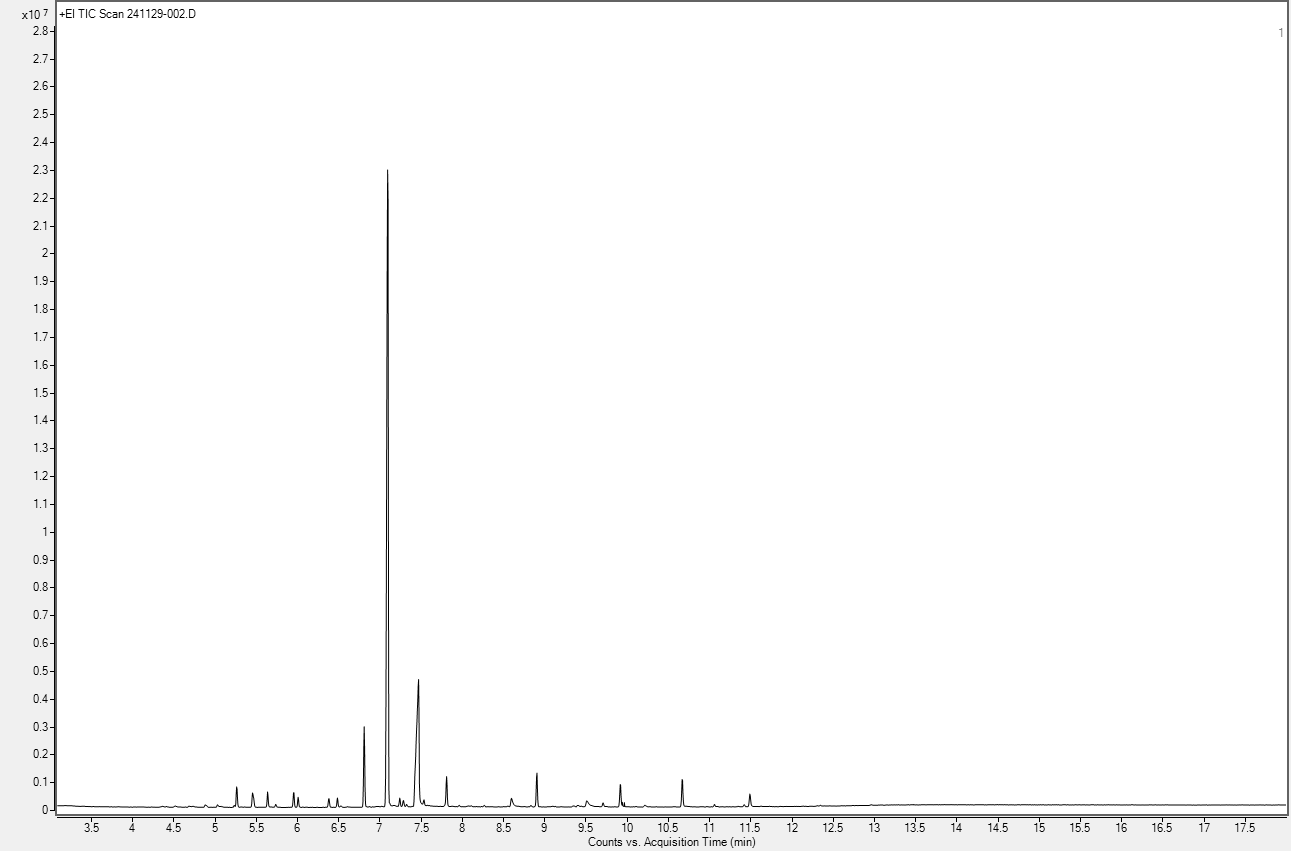
\includegraphics[width=1\linewidth]{graphics/data/GC/241129-002.png}
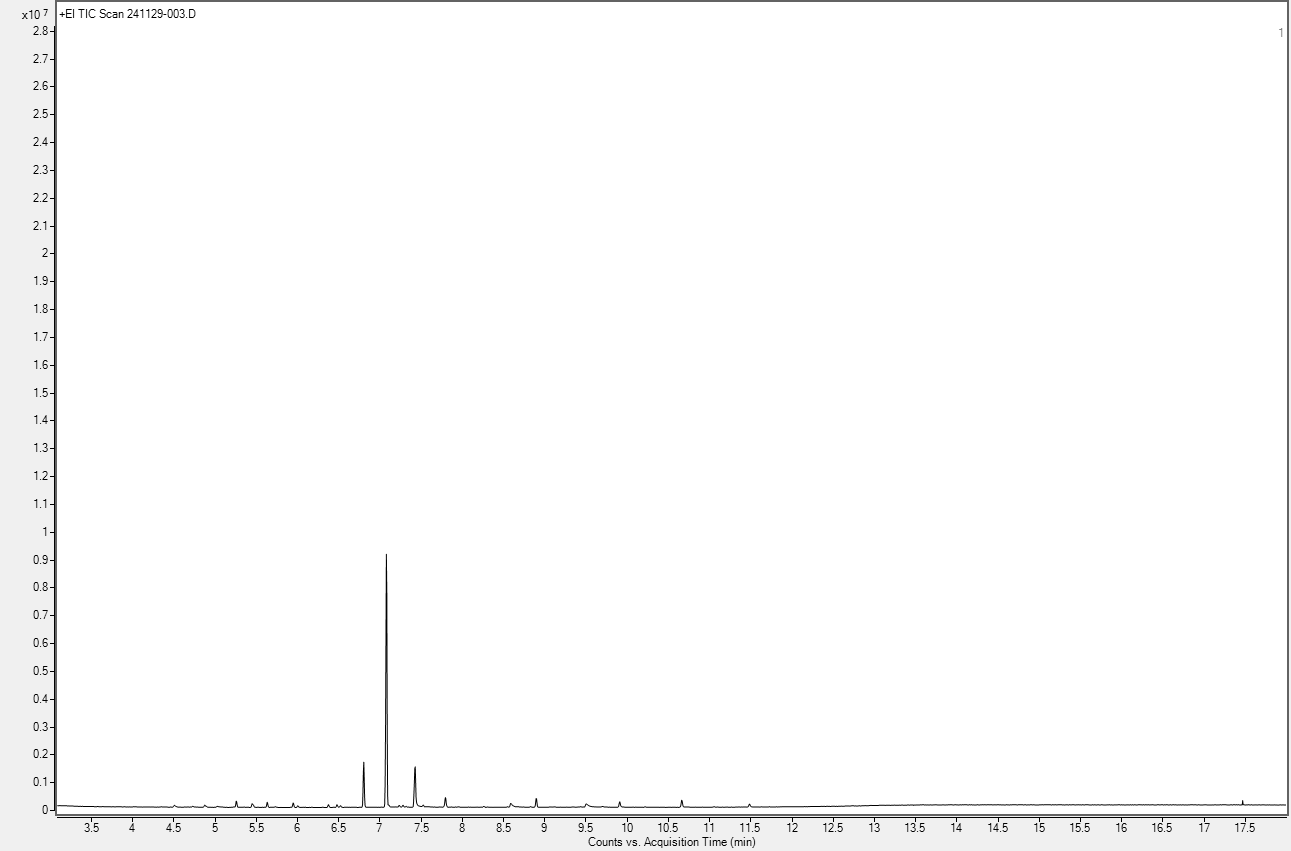
\includegraphics[width=1\linewidth]{graphics/data/GC/241129-003.png}
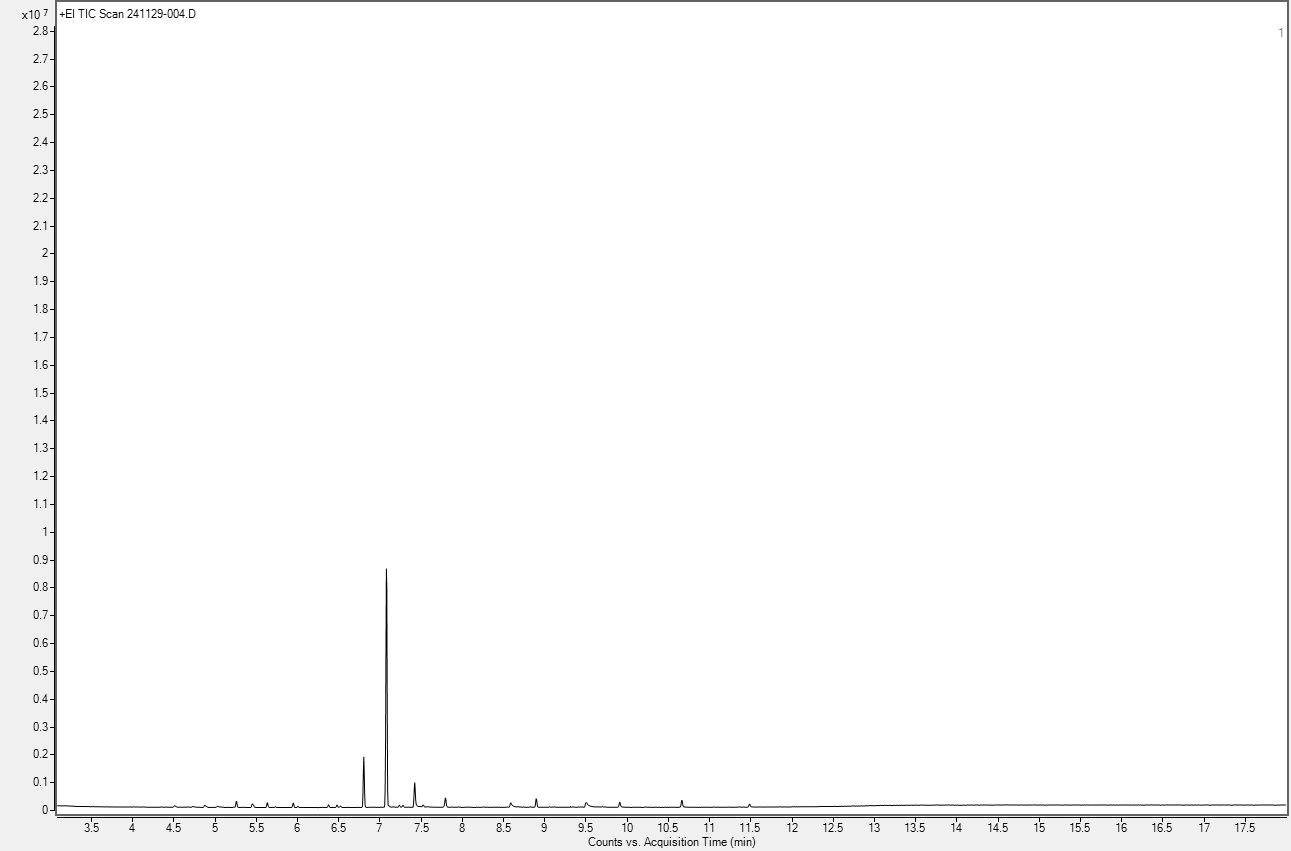
\includegraphics[width=1\linewidth]{graphics/data/GC/241129-004.png}
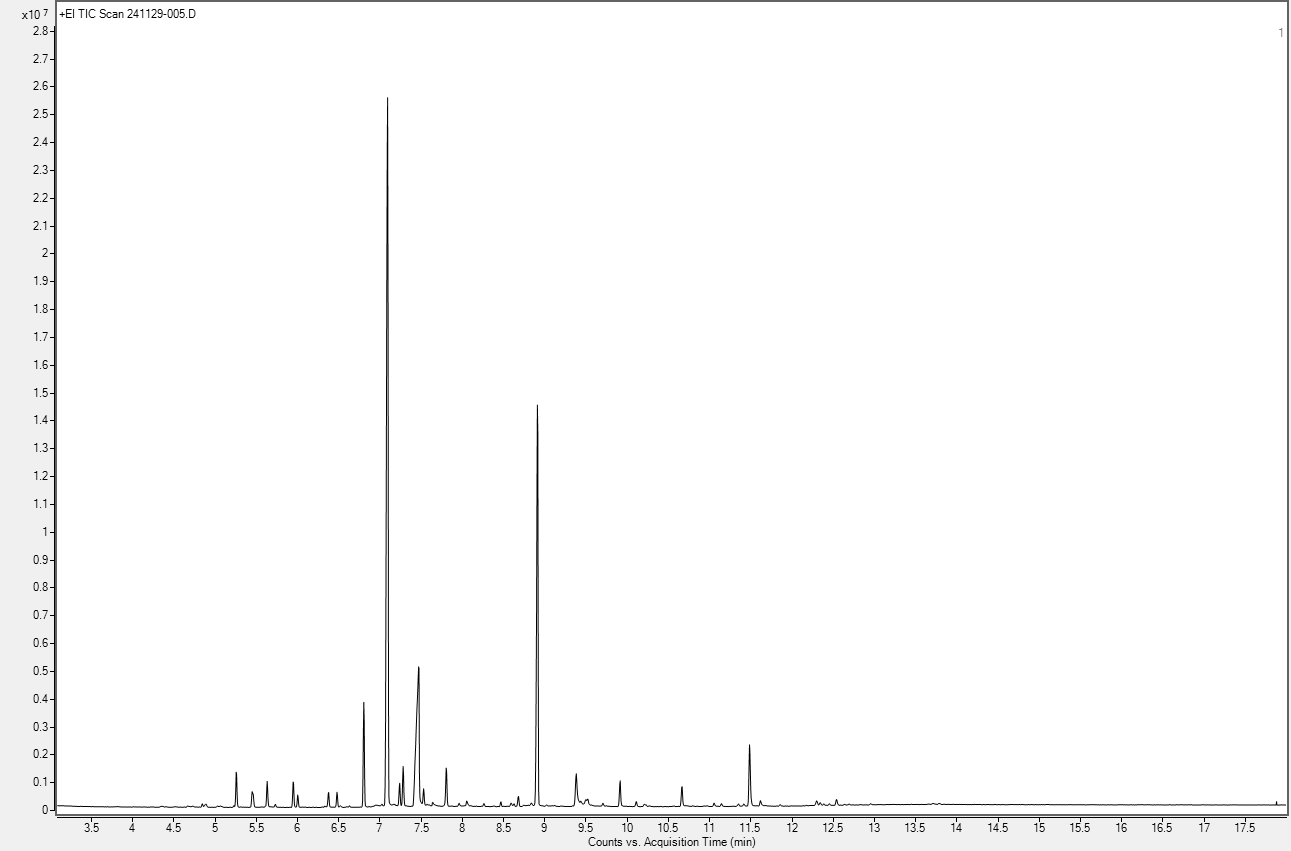
\includegraphics[width=1\linewidth]{graphics/data/GC/241129-005.png}
\newpage\subsection{Massespektre}
Her vises massespektre brugt til identifikation i \cref{tab:id-substance}. Baggrundsstøj er forsøgt fjernet.\par
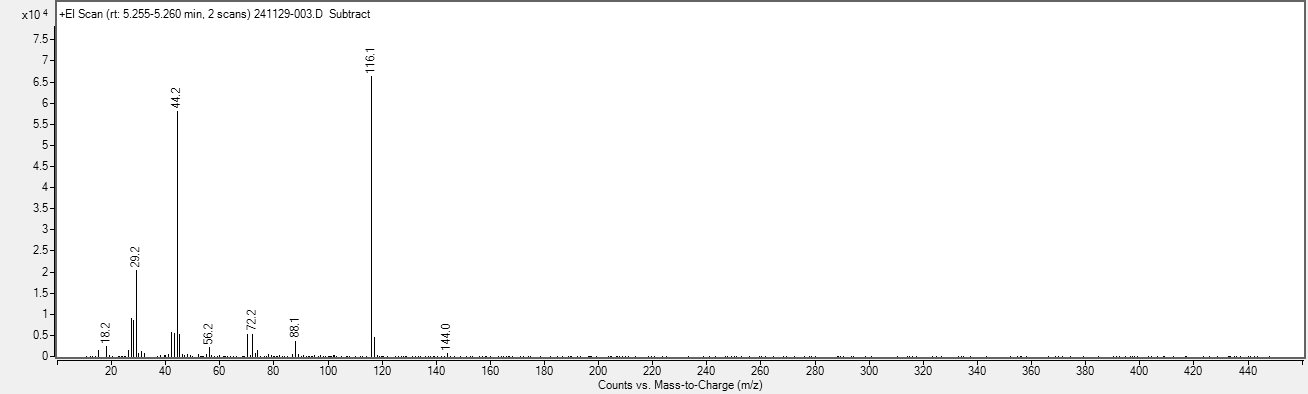
\includegraphics[width=1\linewidth]{graphics/data/MS/05255.png}
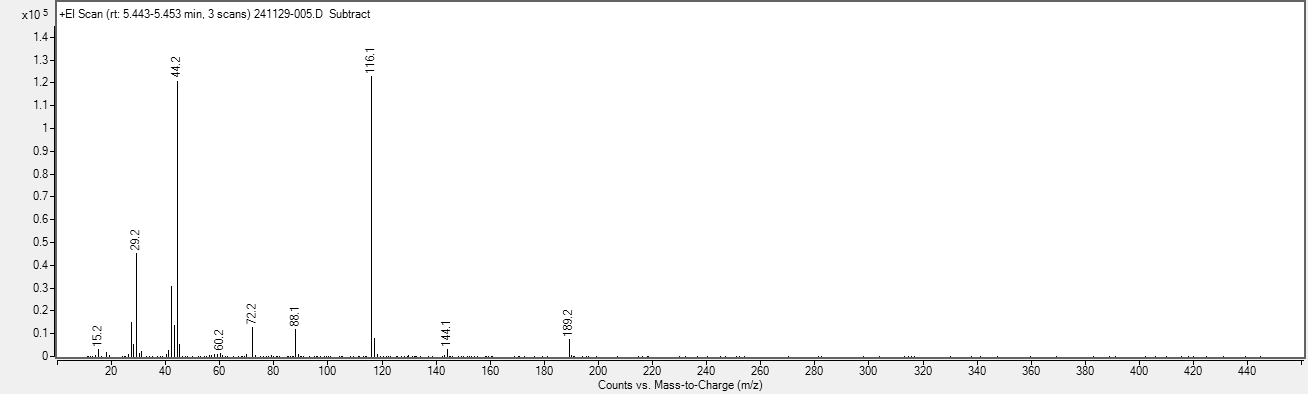
\includegraphics[width=1\linewidth]{graphics/data/MS/05448.png}
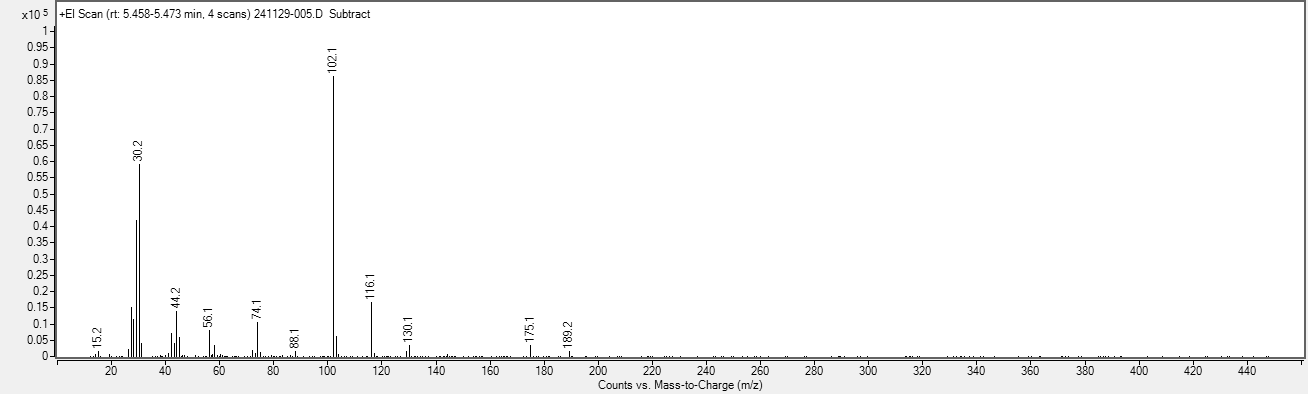
\includegraphics[width=1\linewidth]{graphics/data/MS/05463.png}
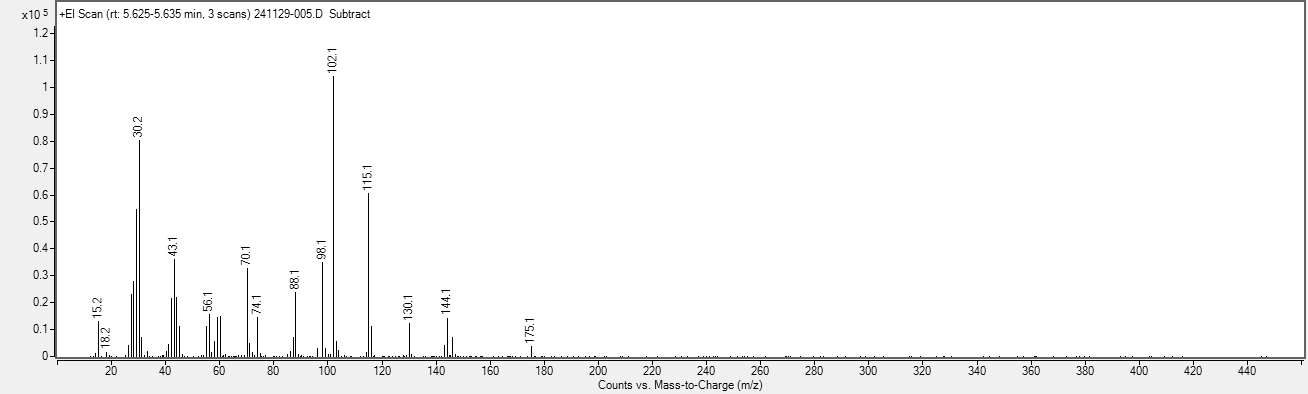
\includegraphics[width=1\linewidth]{graphics/data/MS/05635.png}
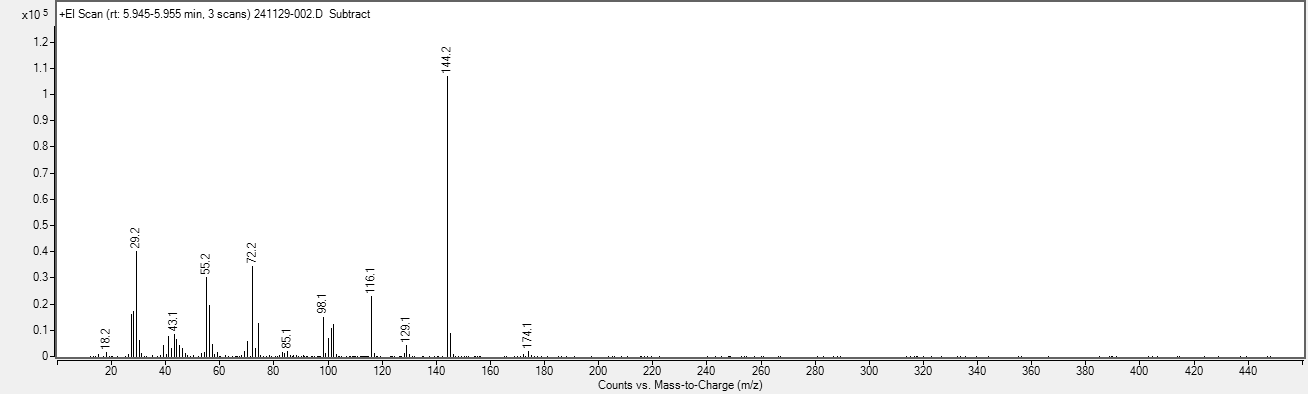
\includegraphics[width=1\linewidth]{graphics/data/MS/05955.png}
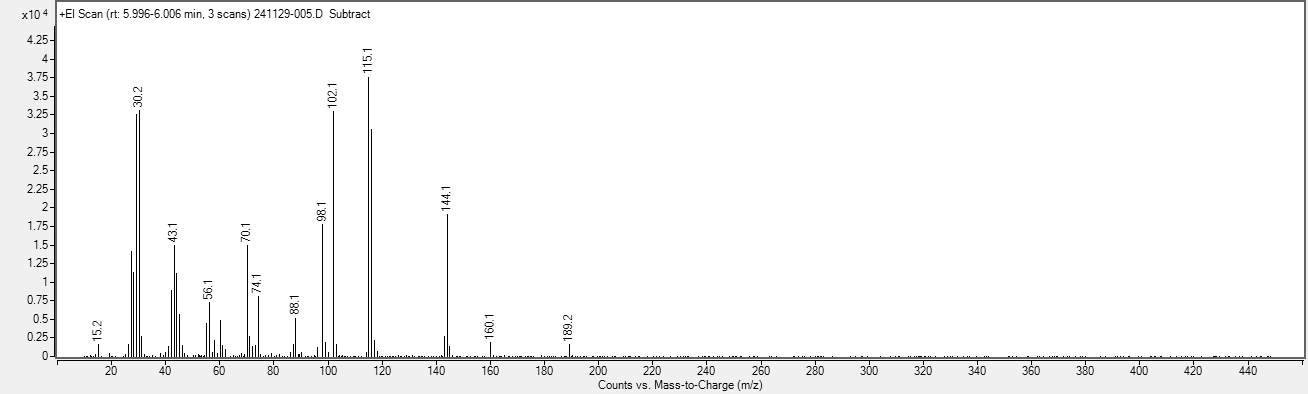
\includegraphics[width=1\linewidth]{graphics/data/MS/06001.png}
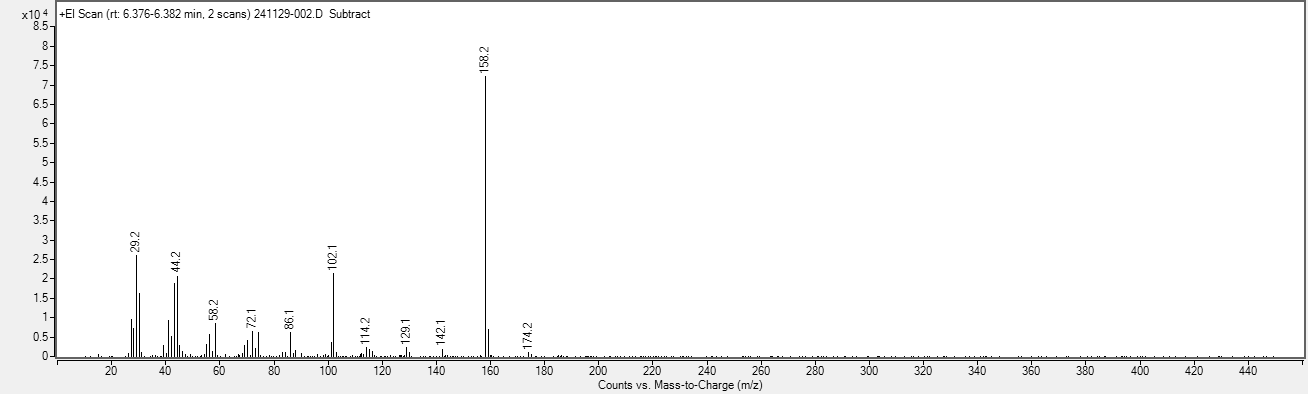
\includegraphics[width=1\linewidth]{graphics/data/MS/06382.png}
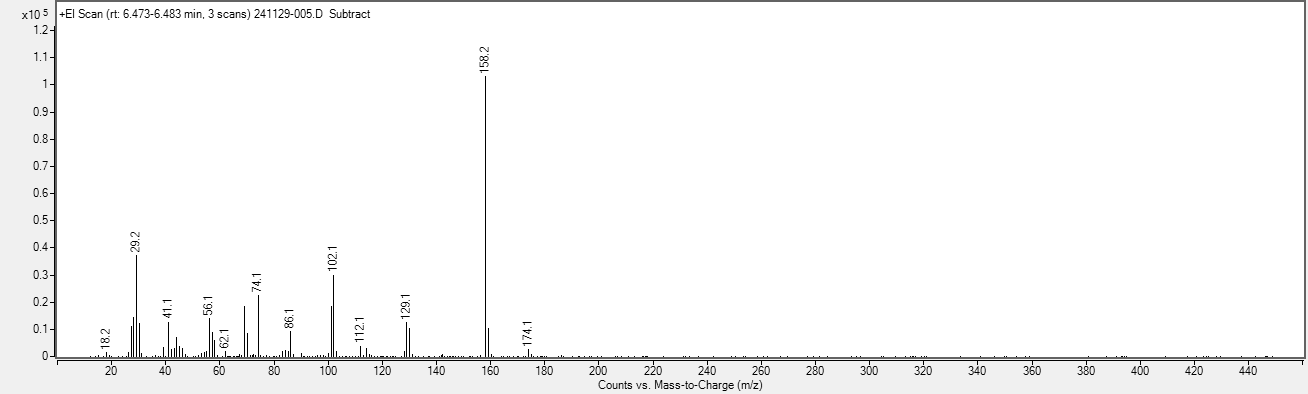
\includegraphics[width=1\linewidth]{graphics/data/MS/06478.png}
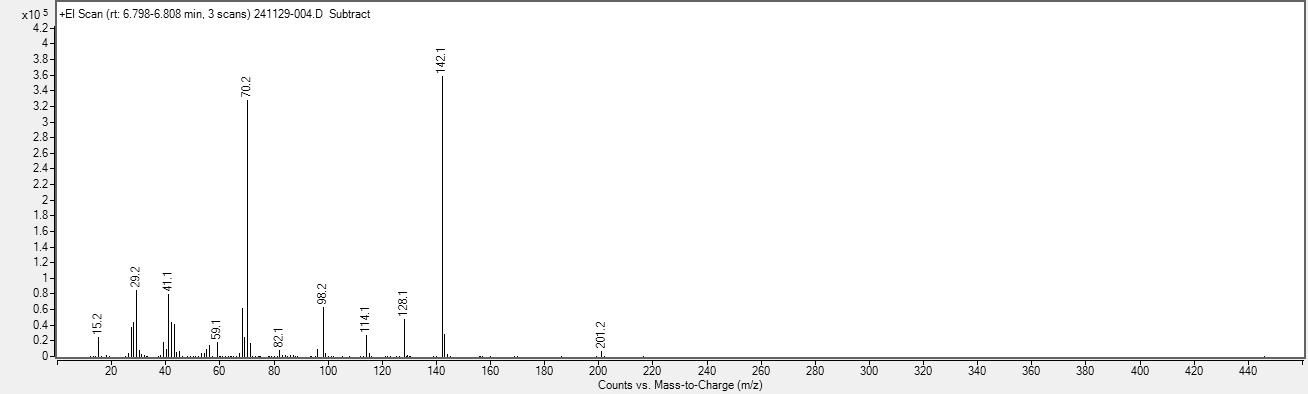
\includegraphics[width=1\linewidth]{graphics/data/MS/06803.png}
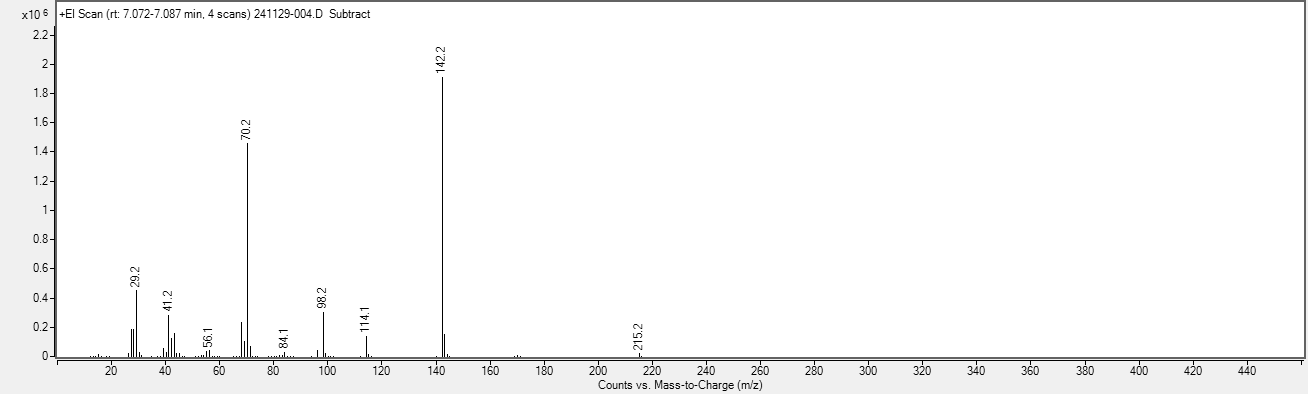
\includegraphics[width=1\linewidth]{graphics/data/MS/07077.png}
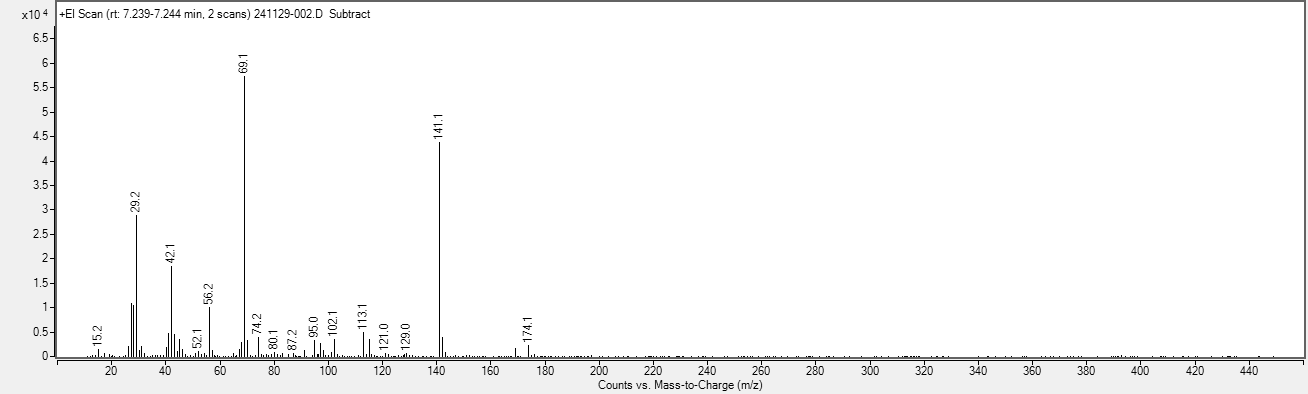
\includegraphics[width=1\linewidth]{graphics/data/MS/07239.png}
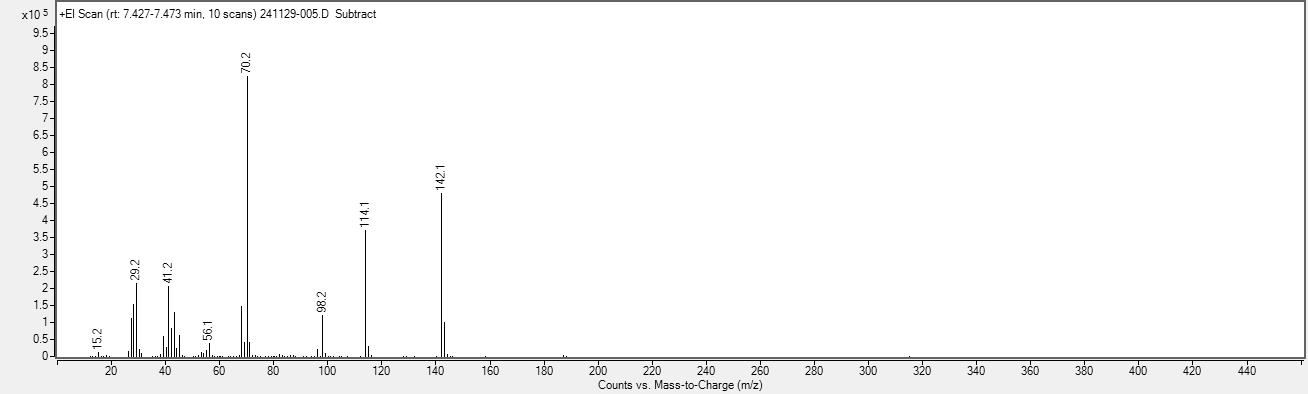
\includegraphics[width=1\linewidth]{graphics/data/MS/07468.png}
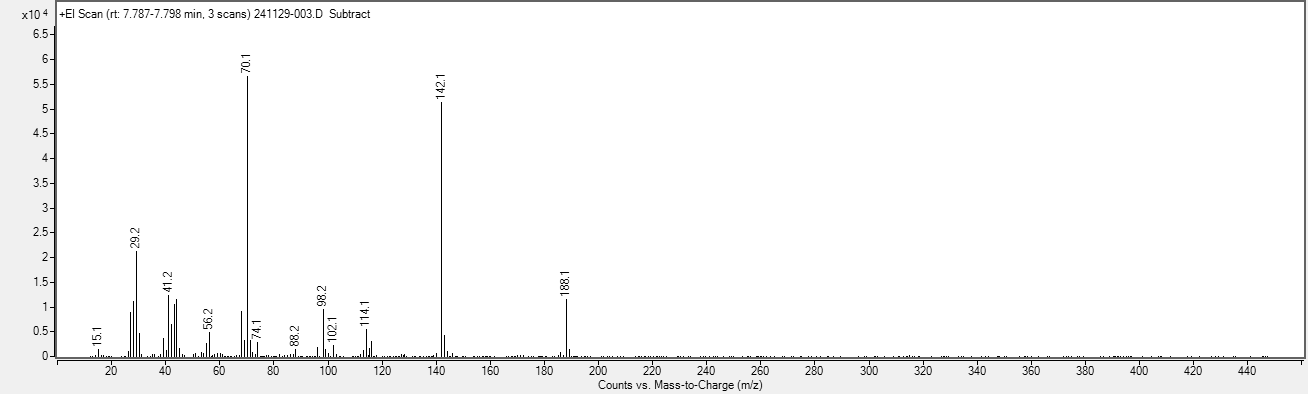
\includegraphics[width=1\linewidth]{graphics/data/MS/07793.png}
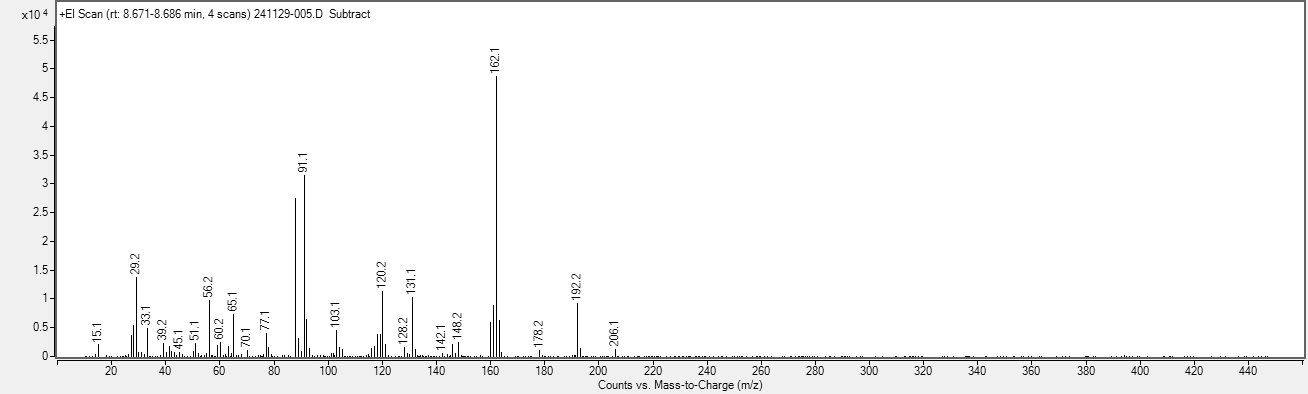
\includegraphics[width=1\linewidth]{graphics/data/MS/08681.png}
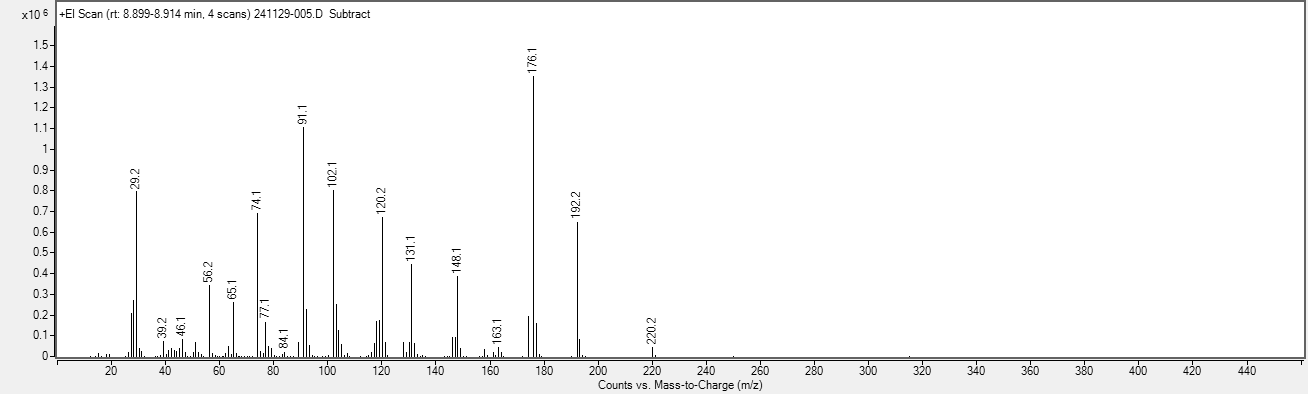
\includegraphics[width=1\linewidth]{graphics/data/MS/08909.png}
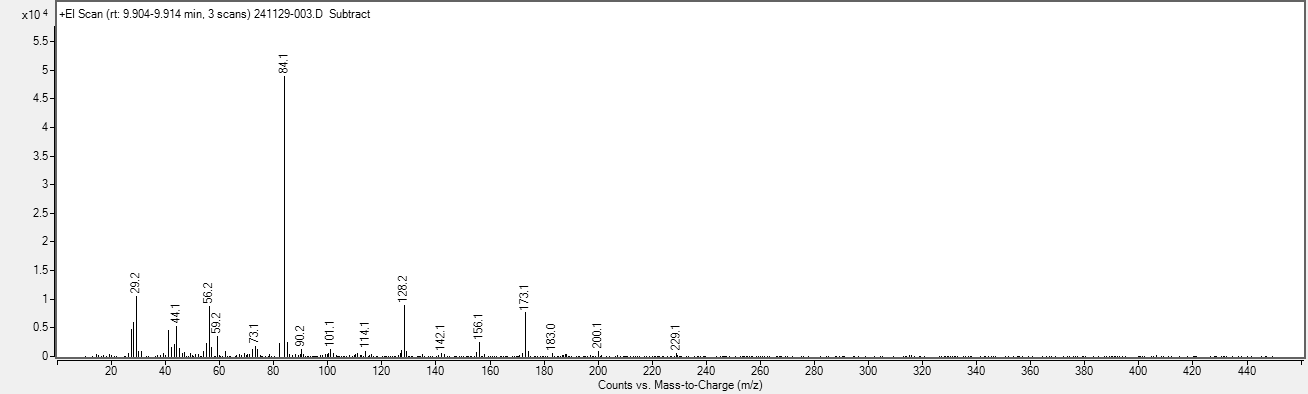
\includegraphics[width=1\linewidth]{graphics/data/MS/09909.png}
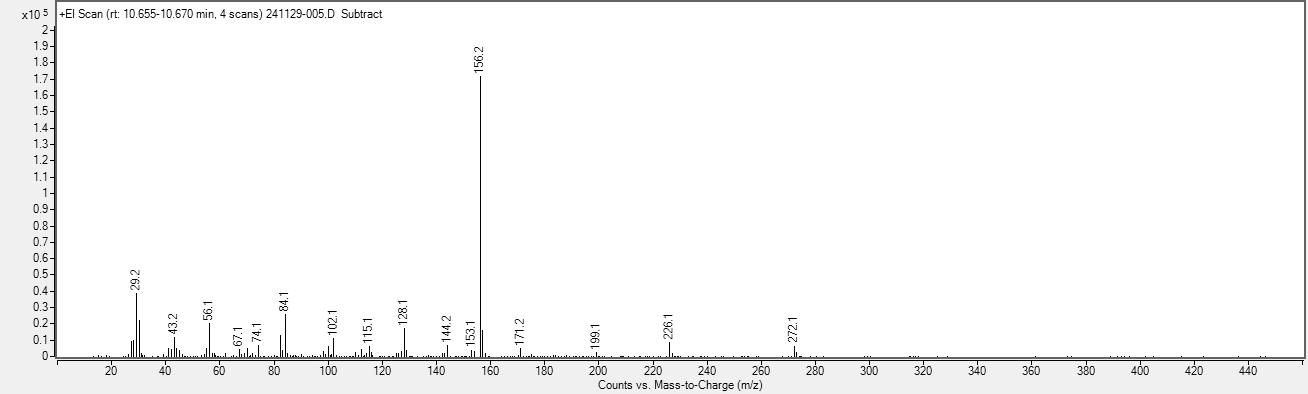
\includegraphics[width=1\linewidth]{graphics/data/MS/10665.png}
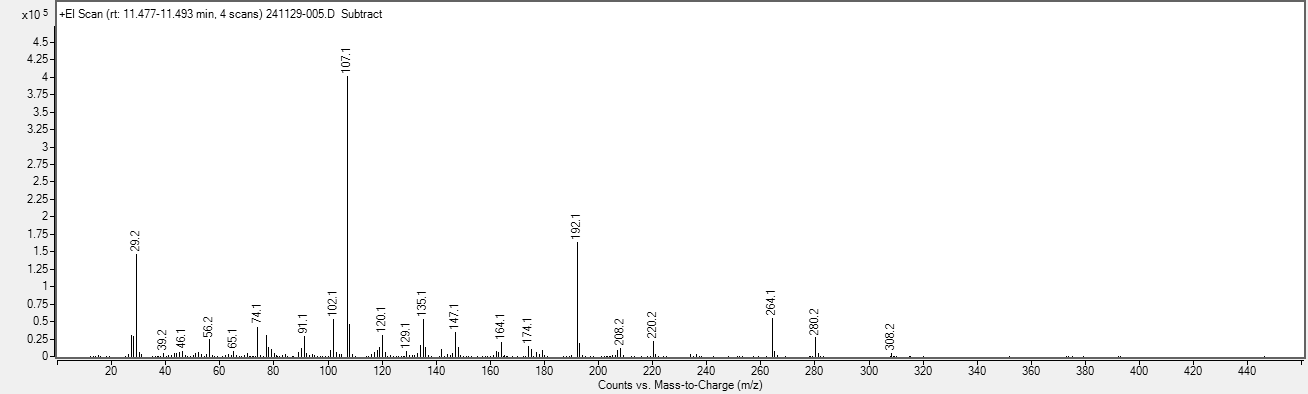
\includegraphics[width=1\linewidth]{graphics/data/MS/11482.png}
